\documentclass[border=10pt]{standalone}

\usepackage{tikz}
\usepackage{tikzsymbols}
\usetikzlibrary{calc,patterns,shapes.geometric}

\def\centerarc[#1](#2)(#3:#4:#5){\draw[#1] ($(#2)+({#5*cos(#3)},{#5*sin(#3)})$) arc (#3:#4:#5);}

\begin{document}
	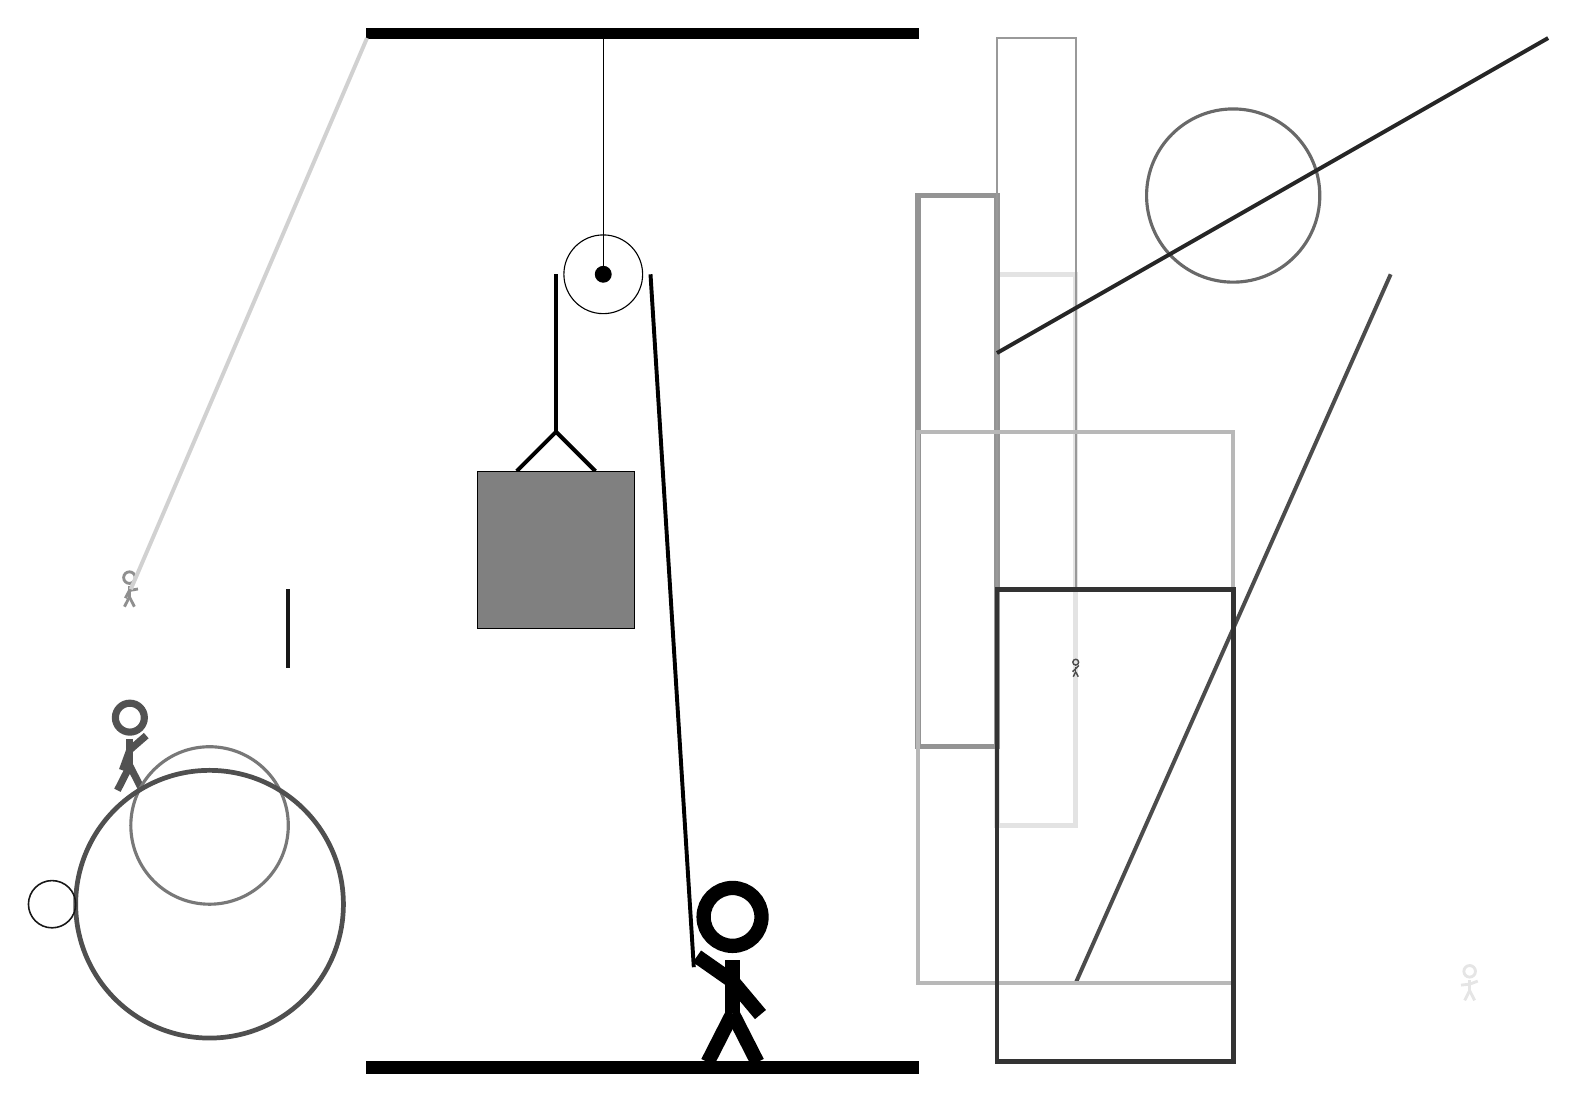
\begin{tikzpicture}
		%%%%% START %%%%%
		
		\draw[fill=black] (-2, 10) rectangle (5, 10.125);
		
		\draw (1, 7) circle (0.5);
		\draw[fill=black] (1, 7) circle (0.1);
		\draw (1, 10) -- (1, 7);
		
		\draw[line width=0.5mm] (-0.1, 4.5) -- (0.4, 5.0) -- (0.9, 4.5);
		\draw[fill=black!50] (-0.6, 4.5) rectangle (1.4, 2.5);
		
		\draw[line width=0.5mm] (0.4, 7) -- (0.4, 5.0);
		\centerarc[line width=0.5mm](1, 7)(0:180:0.6);
		\draw[line width=0.5mm](1.6, 7) -- (2.15, -1.8);
		
		\draw[line width=0.7mm, color=black!11] (7, 7) rectangle (6, 0);
		
		\draw [line width=0.4mm, color=black!59](9, 8) circle (1.1);
		\draw[line width=0.5mm, color=black!91](-3, 2) -- (-3, 3);
		\node[line width=0.7mm, color=black!10] at (12, -2) {\Strichmaxerl[2][6][21]};
		
		\node[line width=0.4mm, color=black!68] at (-5, 1) {\Strichmaxerl[5][70][41]};
		\node[line width=0.2mm, color=black!70] at (7, 2) {\Strichmaxerl[1][44][45]};
		\draw [line width=0.4mm, color=black!53](-4, 0) circle (1.0);
		
		\node[line width=0.4mm, color=black!44] at (-5, 3) {\Strichmaxerl[2][62][10]};
		\draw [line width=0.6mm, color=black!69](-4, -1) circle (1.7);
		
		\draw[line width=0.7mm, color=black!42] (6, 8) rectangle (5, 1);
		\draw[line width=0.5mm, color=black!40](7, -2) -- (7, -2);
		\draw[line width=0.2mm, color=black!40] (6, 3) rectangle (7, 10);
		\draw[line width=0.5mm, color=black!85](6, 6) -- (13, 10);
		\draw[line width=0.5mm, color=black!70](7, -2) -- (11, 7);
		\draw [line width=0.2mm, color=black!91](-6, -1) circle (0.3);
		\draw[line width=0.5mm, color=black!18](-5, 3) -- (-2, 10);
		
		\draw[line width=0.5mm, color=black!28] (5, -2) rectangle (9, 5);
		\draw[line width=0.6mm, color=black!80] (6, -3) rectangle (9, 3);
		
		\node at (2.6, -1.9) {\Strichmaxerl[10][-35][-50]};
		
		\draw[fill=black] (-2, -3) rectangle (5, -3.15);
		
		%%%%% END %%%%%
	\end{tikzpicture}
\end{document}